\chapter{Resultados}
\label{chap:result}

As funcionalidades do sistema de percepção foram validadas a partir de duas etapas de testes. Os testes unitários buscam a validação do funcionamento individual dos sensores, enquanto os testes integrados validam o funcionamento dos sistemas e funcionalidades, ou seja, todos os componentes em conjunto. A descrição dos testes realizados e dos resultados obtidos por eles está descrita abaixo.

Para mais detalhes sobre as conexões eletro-eletrônicas, pode-se ver o apêndice \ref{Append:diagele}.

%--------- NEW SECTION ----------------------
\section{Testes unitários}
\label{sec:testu}

	\subsection{Câmera Térmica}
	
		A câmera térmica Lepton, do fabricante FLIR, se comunica por VOSPI. Logo, foi necessário utilizar um driver para converter os dados da câmera e disponibiliza-los para a USB. Uma placa de desenvolvimento Nucleo STM32F401RE com o driver disponibilizado por \citeonline{groupgets} foi utilizada para essa situação.
		
		\begin{figure}[!ht]
		   \centering
		   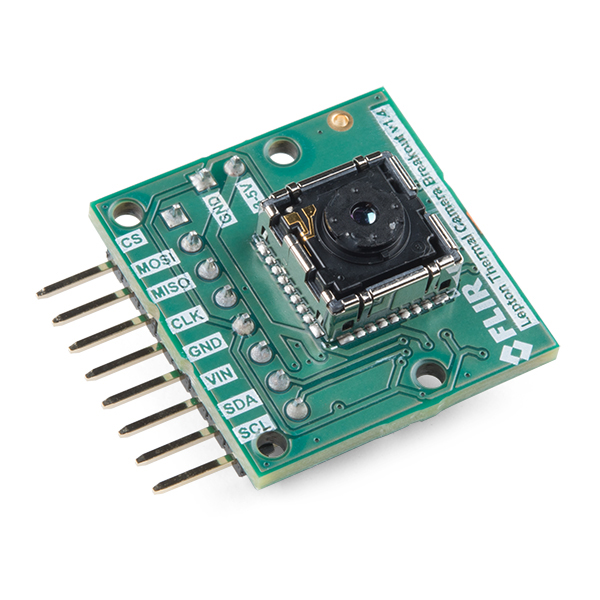
\includegraphics[width=6cm]{Figures/lepton_flir.jpg}
		   \caption{Lepton LWIR}
		   \label{fig:lepton}
		\end{figure}
		
		O driver coleta os frames e verifica se o mesmo foi adquirido corretamente, após isso, envia para a USB seguindo o seguinte padrão de mensagem:
		    
		\begin{figure}[!ht]
		   \centering
		   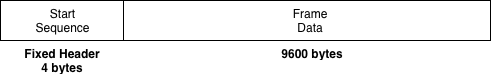
\includegraphics[width=14cm]{Figures/frame_msg.png}
		   \caption{Mensagem do frame da câmera}
		   \label{fig:framemsg}
		\end{figure}
	
	    No início de cada mensagem, há uma sequência de quatro \textit{bytes} para confirmar a transferência dos dados. Após a confirmação por um \textit{script} em python, inicia-se o processo de aquisição do \textit{frame}. Cada \textit{frame} é composto por 4800 \textit{pixeis}, sendo 80 na horizontal e 60 na vertical. Além disso, cada \textit{pixel} possui 2 \textit{bytes} de profundidade de cor, correspondendo a 9600 \textit{bytes} de informação para cada \textit{frame}. Na Figura \ref{fig:frame_esque}, pode-se observar uma representação do \textit{frame} da câmera.
	    
	%\pagebreak
	
		\begin{figure}[!ht]
		   \centering
		   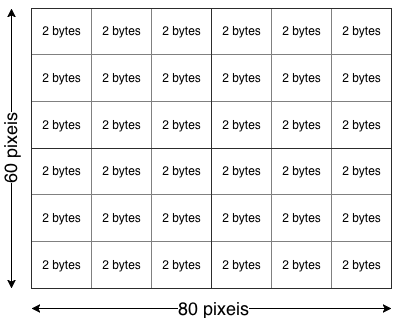
\includegraphics[width=10cm]{Figures/frame_esque.png}
		   \caption{Esquemático do \textit{Frame} da Câmera Térmica}
		   \label{fig:frame_esque}
		\end{figure}
		
		No \textit{script} de aquisição de \textit{frames}, cada \textit{pixel}, foi convertido para uma escala de cinza de 8-bits (1 \textit{byte}). Conversão necessária para trabalhar com a biblioteca de processamento de imagens OpenCV.
		    
		Após isso a imagem foi reconstruída para verificar a integridade dos \textit{frames}.
	
	\subsection{Sonar EZ-1}
		O sonar EZ-1 da MaxBotix possui saída analógica referente a distância medida. Para testa-lo, foi utilizada uma das entradas analógicas da Phidgets.
		
		\pagebreak
		
		\begin{figure}[!ht]
		   \centering
		   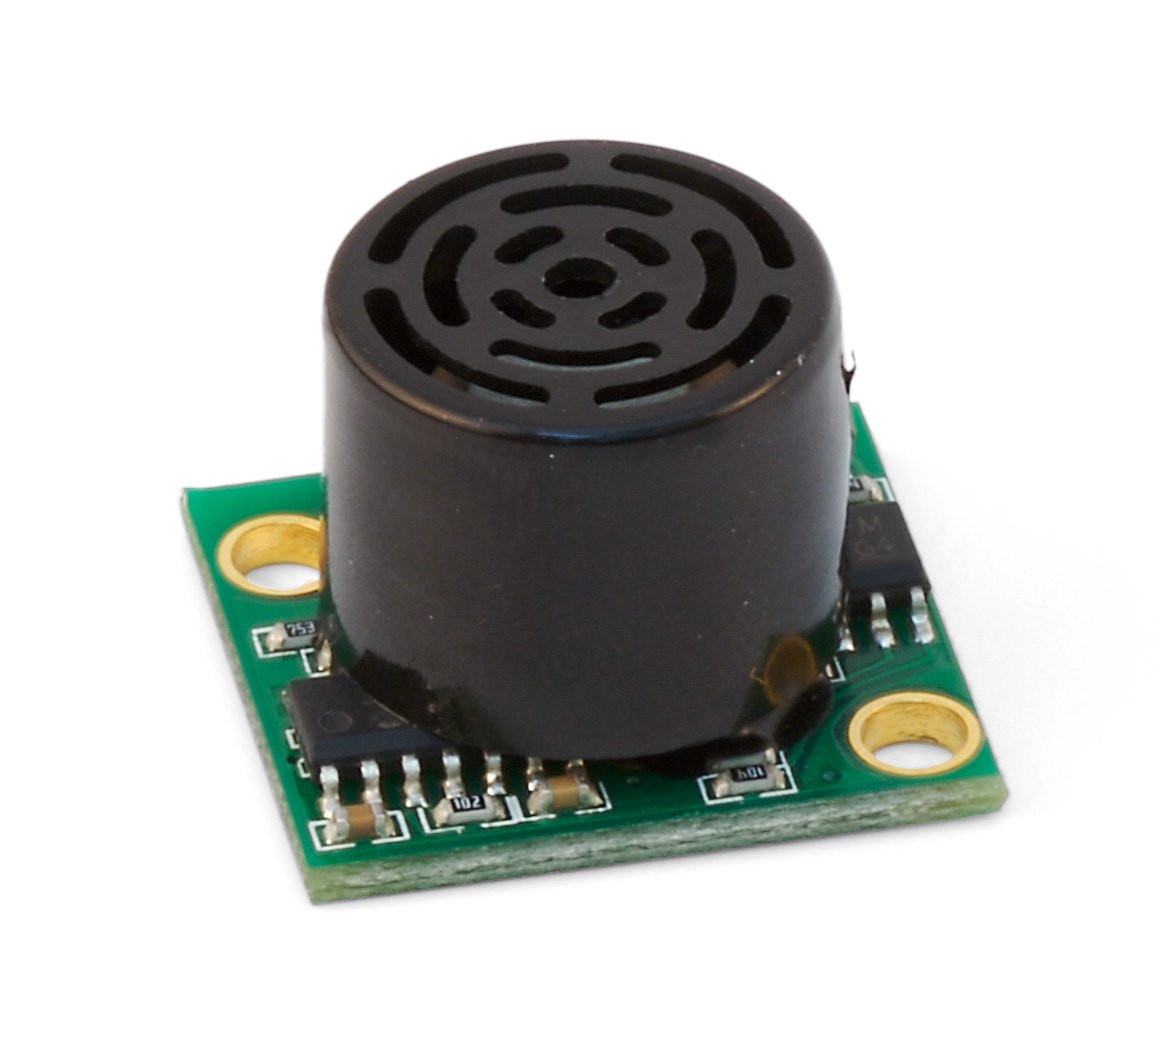
\includegraphics[width=8cm]{Figures/ez1.jpg}
		   \caption{Sonar EZ-1}
		   \label{fig:ez1}
		\end{figure}
		
		A comunicação da Phidgets com com a NUC é feita via USB, contudo, é necessário a instalação dos drivers obrigatórios da placa no linux. Além disso, é necessário a instalação do módulo python respectivo da placa, dessa forma, permitindo a utilização de classes e métodos para controle da comunicação com os sensores.
		
		Com os respectivos drivers e módulos da phidgets instalados no computador, foi necessário apenas conectar os terminais alimentação e saída analógica do sensor nos conectores correspondentes da Phidgets e executar um \textit{script} de leitura da tensão nas entradas analógicas fornecido pela própria fabricante. 
		
		Ao executar o código, recebe-se, no intervalo de dez segundos, todas as leituras de tensão efetuadas no sensor. Notamos que ao afastar o obstáculo do sonar o valor de tensão aumentava e quando aproximavamos o obstáculo o valor de tensão diminuía. Após feita a conversão de tensão para unidades métricas através das informações disponibilizadas no \textit{datasheet}, foi possível validar o sensor.
	
	\subsection{Sensor de Proximidade}
		O sensor de proximidade E18-D80NK funciona de maneira bastante simples. O módulo possui um emissor e um receptor de feixes infra-vermelhos, o qual identifica se há ou não um objeto próximo devido a reflexão, liberando assim, um sinal de nível alto caso positivo e nível baixo caso negativo.
		
		\begin{figure}[!ht]
		   \centering
		   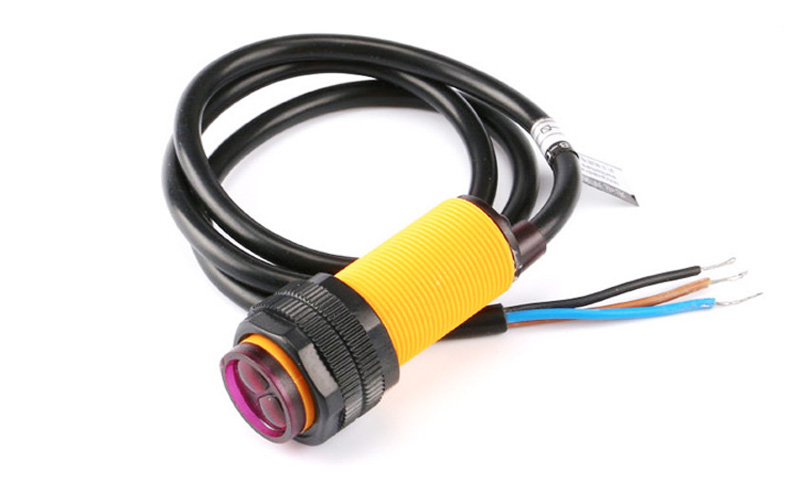
\includegraphics[width=8cm]{Figures/proximity_sensor.jpg}
		   \caption{Sensor de proximidade E18-D80NK}
		   \label{fig:E18-D80NK}
		\end{figure}
		
		Por questão de sinalização, o fabricante adicionou um LED, que ao identificar algum objeto próximo, acende-se. Com isso, logo após alimentar o sensor já era possível ver o seu funcionamento. Entretanto, ainda era necessário verificar se a saída digital referente a detecção estava em devido funcionamento.
		
		Para isso, foi utilizada a placa de interfaceamento Phidgets assim como no tópico anterior. O que diferiu nesse teste para o anterior é que o sensor foi acoplado em uma entrada digital, em vez de uma analógica, assim como o \textit{script} executado foi para comunicação com as entradas digitais. O código, também disponibilizado pela fabricante, notifica a mudança de estado da saída dos sensor, dessa maneira podendo ser validada.
		
	\subsection{\textit{Smart Charger}}
    
	    A placa de gerenciamento e carregamento das baterias DS325A, da empresa Inspired Energy, funciona a partir do protocolo de comunicação SMBus. Informações das baterias como temperatura, corrente, carga, entre outras podem ser solicitadas através do seguinte protocolo de leitura.
	    
	    \begin{figure}[!ht]
			   \centering
			   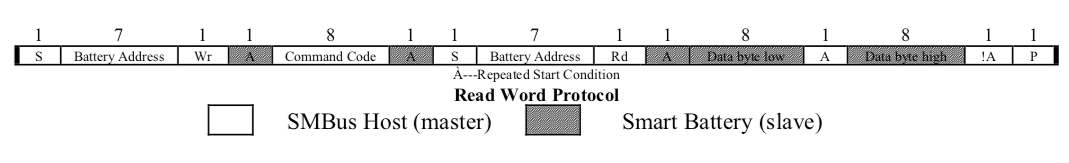
\includegraphics[width=16cm]{Figures/batt_protocol.png}
			   \caption{Protocolo de comunicação do \textit{Smart Charger} e das baterias}
			   \label{fig:batt_protocol}
		\end{figure}   
		
		No qual é necessário enviar primeiro o endereço de 7 bits da bateria de interesse, seguido do comando referente a que informação está se requisitando. Após isso, inicia-se o processo de leitura das informações da bateria.
		
		O driver de comunicação foi desenvolvido em uma placa de desenvolvimento Nucleo STM3L432KC para disponibiliza-los na USB do computador. Além disso, um \textit{script} em python foi escrito para requisitar essas informações do microcontrolador.
	    
	    Os dados foram convertidos para suas respectivas grandezas, dessa maneira, foi possível validar as informações obtidas.
    
    \subsection{Sensor de Temperatura}
    
	    O sensor de temperatura LM35 possui uma saída analógica e com comportamento linear entre a tensão de saída e a temperatura medida.
	    
	    \begin{figure}[!ht]
			   \centering
			   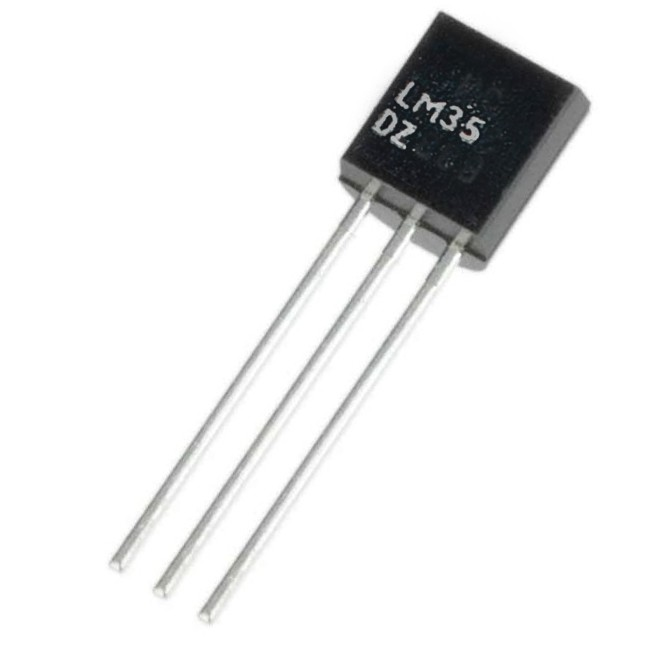
\includegraphics[width=6cm]{Figures/lm35.jpg}
			   \caption{Sensor de Temperatura LM35}
			   \label{fig:LM35}
		\end{figure}
	   
	    O componente foi testado em uma das entradas analógicas da Phidgets, e utilizando o mesmo algoritmo de leitura de tensão já mencionado para realizar a obtenção de dados. Para verificar a resposta do sensor, foi medido o valor de tensão de saída para uma sala com ar-condicionado e para um ambiente externo com auxílio de um termômetro de referência.
	    
	    Os valores de tensão foram convertidos para graus Celsius, através da correlação disponível no \textit{datasheet}, validando assim o sensor.
    
    \subsection{GPS}
    
	    O GPS Piksi v2.3.1, da Swift Navigation, possui um console disponibilizado pelo próprio fabricante, porém como se tinha em mãos uma versão antiga do aparelho, foi necessário descobrir qual a versão compatível do \textit{software}.
	    
	    \begin{figure}[!ht]
				   \centering
				   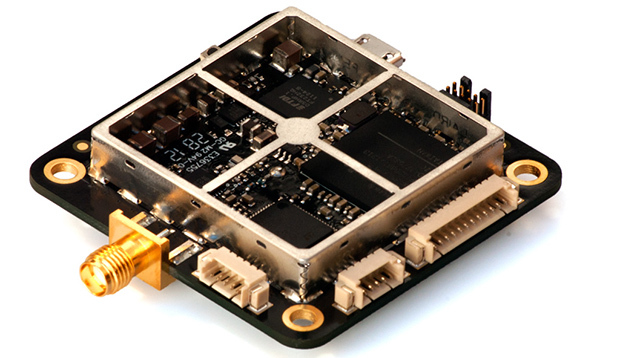
\includegraphics[width=6cm]{Figures/gps.jpg}
				   \caption{GPS Piksi v2.3.1}
				   \label{fig:GPS}
		\end{figure}
			    
	     O console foi instalado, o GPS foi conectado na USB do computador e a antena devidamente acoplada. Essa versão em específico precisa de quatro satélites para realizar os cálculos de coordenadas, e em ambientes fechados, a recepção de sinal é bastante degradada. Para contornar essa situação, o dispositivo foi iniciado em modo de simulação em seu console, mostrando assim, os dados de longitude e latitude.
	     
	     Posteriormente, a antena foi levada a um ambiente externo e verificou o funcionamento do GPS fora do modo de simulação.    

	\subsection{IMU}
	    
	    A IMU Mti-1, fabricado pela Xsens, possui um console que é disponibilizado no próprio pendrive de instalação que vem junto ao sensor.
	    
	    \begin{figure}[!ht]
		   \centering
		   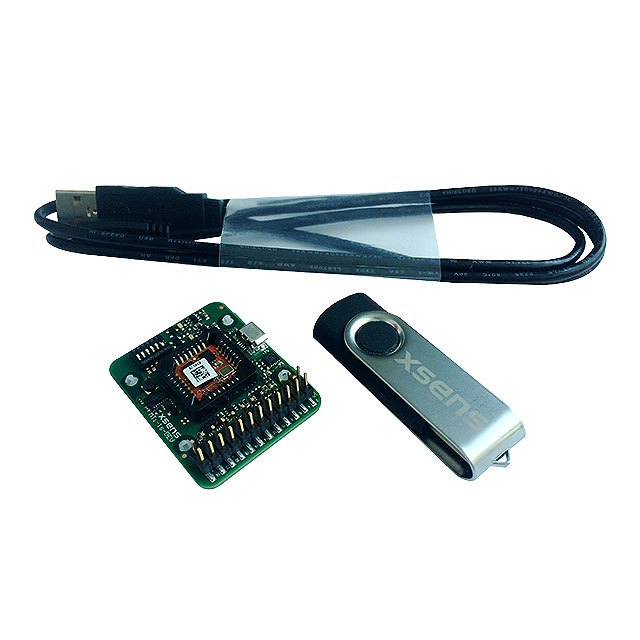
\includegraphics[width=8cm]{Figures/imu.jpg}
		   \caption{IMU Xsens Mti-1}
		   \label{fig:IMU}
		\end{figure}
	    
	     Com o console instalado, foi apenas necessário conectar a IMU a uma das portas USB do computador. Na própria interface gráfica já aparece as informações de orientação do dispositivo, informando a orientação nos três eixos de referência e velocidade angular.
	
%--------- NEW SECTION ----------------------
\section{Integração no ROS}
\label{sec:rosinte}

	Após os testes unitários de cada sensor, deu-se inicio à integração dos sensores no ambiente ROS para construção do sistema de Percepção. A descrição da metodologia empregada para embarcar cada um dos sensores no framework de robótica está mostrada nos tópicos abaixo.

\subsection{Phidgets}
     Após a fase de testes unitários, foi necessário desenvolver o \textit{package} de comunicação da phidgets no ROS. Esse \textit{package} é responsável pela aquisição dos dados de todos os sensores analógicos e digitais conectados a Phidgets.
     
     Os nós foram desenvolvidos utilizando como base o módulo \textit{python} da Phidgets. Ele consiste em uma classe e cada objeto desta, representa um componente conectado a placa de interface. Ao declarar o objeto, se faz necessário informar o canal, o nome do dispositivo, o tipo de porta (digital ou analógico) e o nome do tópico a ser disponibilizado os dados. 
     
     No construtor da classe os dados referentes aos dispositivos são coletados e um \textit{publisher} do ROS é inicializado. Este  \textit{publisher} faz com que periodicamente os dados de tensão(canais analógicos) ou status da porta(canais digitais) sejam coletados e disponibilizados no tópico escolhido pelo usuário. 
     
     No script original foram criados seis objetos da classe no \textit{main loop}, correspondentes aos cinco sensores de proximidade conectados a portas digitais e ao sonar conectado na porta analógica.
     
\subsection{Smart Charger}
     
     O script utilizado no teste unitário para receber os dados provenientes do \textit{smart charger} no computador foi utilizado como base para a construção do nó no ambiente ROS.
     
     O nó funciona enviando um \textit{byte} pré-definido para dar início ao processo de transmissão de dados da bateria. A recepção do \textit{byte} pela Nucleo L432KC inicia a leitura dos dados da bateria, como mostrado no tópico anterior. Logo após isso, ocorre o envio das informações em sequência para o computador, como pode ser visto abaixo:
      
      \begin{figure}[!ht]
		   \centering
		   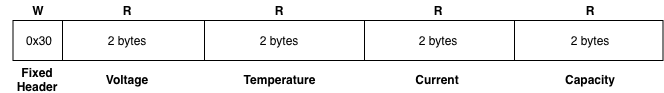
\includegraphics[width=16cm]{Figures/batt_protocol_2.png}
		   \caption{Mensagem entre a Nucleo L432KC e o nó referente às baterias}
		   \label{fig:battprotocol2}
		\end{figure}
		      
      No nó do ROS essas informações são recebidas via serial e convertidas para sua devidas unidades segundo o \textit{datasheet} do fabricante. Esses dados são colocados em um formato de mensagem chamado de Battery e publicadas em um tópico do ROS. O nó criado para a \textit{smart charger} está mostrado no anexo XX.
     
     \subsection{Câmera Térmica}
     
     A integração da câmera no ROS foi feita em duas etapas, que na prática foram representadas como dois nós:
     
     \begin{itemize}
         \item O primeiro com objetivo da aquisição dos dados da câmera e sua disponibilização em um tópico.
         \item O segundo nó é responsável por todo o tratamento da imagem e detecção dos pontos quentes.
     \end{itemize}
     
     Para a aquisição dos dados, no primeiro nó, foi utilizado basicamente o mesmo algoritmo que no teste unitário, porém com a integração das bibliotecas do ROS para publicar os \textit{frames} em forma de \textit{Numpy arrays} em seus devido tópico.
     
     No segundo nó foi utilizado a biblioteca OpenCV para realizar o processamento da imagem. Primeiramente, o frame disponibilizado pelo nó de aquisição é adquirido subscrevendo do seu respectivo tópico. Para retirar o aspecto "pixelado" da imagem da câmera, devido a sua baixa resolução (80x60 pixeis), foi necessário realizar uma interpolação cúbica para redimensionar a imagem para uma resolução de (400x300 pixeis), obtendo assim uma imagem mais detalhada. 
     
     Com a imagem já redimensionada, é aplicado um filtro \textit{blur} para eliminar altas frequências que podem interferir na binarização (\textit{thresholding}) que será feita na imagem.
     
     Após o filtro, o frame é binarizado com o objetivo de facilitar a identificação dos pontos quentes através de um algoritmo de busca de contornos.
     
     O esquemático abaixo mostra simplificadamente o processo de tratamento da imagem.
     
    \begin{figure}[!ht]
    	\centering
    	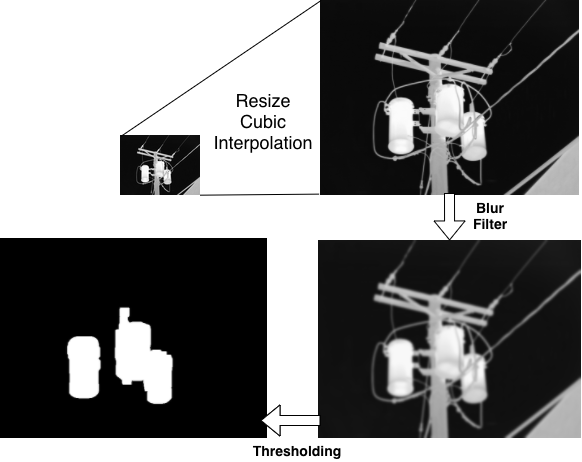
\includegraphics[width=14cm]{Figures/image_proc.png}
    	\caption{Esquemático do processamento da imagem} \label{imgproc}
	\end{figure}
     
     \subsection{GPS}
     
     Para o GPS, foi utilizado um driver disponibilizado no GitHub por \citeonline{ethz} com licensa livre para embarcar o dispositivo no ROS.
     
     O \textit{package} possui nós que publicam em tópicos as informações de coordenadas obtidas do GPS.
     
     \subsection{IMU}
    Foi utilizado o driver da IMU disponibilizada pela própria fabricante Xsens para embarcar a IMU no ROS. O driver de licença livre é disponibilizado no GitHub da própria empresa.
%--------- NEW SECTION ----------------------
\section{Testes integrados}
\label{sec:testi}
asdfadsfsdfs

%--------- NEW SECTION ----------------------
\section{Avaliação da prontidão tecnológica}
\label{sec:trl}
asdfadsfsdfs

%--------- NEW SECTION ----------------------
\section{Trabalhos futuros}
\label{sec:trabfut}
asdfadsfsdfs




